\documentclass{mm2}
\usepackage{bbm}
\usepackage{amsmath}
\usepackage{bbold}
\usepackage{multicol}


% FILL THIS WITH YOUR CIS USERNAME
\cisid{bzqs27} 
\title{Computer Graphics}
\begin{document}


\section{Part 1}
\begin{enumerate}
\item Describe how an index buffer object improves the use of a vertex buffer object in order to represent a 3D mesh.\\ 
\\
\begin{figure}[ht]
	\centering
	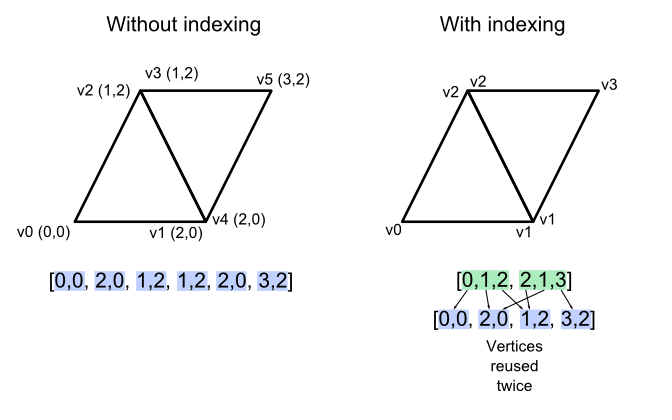
\includegraphics[width=6cm]{INDEXING.PNG}
	\caption{Diagram exhibiting the benefits of an index buffer.}
\end{figure}

\subitem When using a vertex buffer alone to draw a shape that reuses its vertices frequently it can often become confusing to program as it involves re-typing the same vertice many times as the vertice must be defined each time it is referenced. Through using an index buffer we are able to provide a reference (index) for each vertice, thus when we next need to use the vertice we can simply use its index. In a 3d mesh when the same vertice must regularly be used (for example in a cube we must connect 4 vertices with each vertex) an index buffer saves a lot of time for the developer as they do not need to define the vertice each time it is used. So far I have only discussed referencing the vertice for construction of objects but also when we change other attributes of the vertex such as the vertex's colour. If we utilise an index buffer we need only change the attribute (e.g colour) once in the program, however with the vertex buffer alone we would need to change the attribute each time it appeared. Thus from this and the diagram above it is clear that the utilisation of an index buffer will reduce both time to develop programs and memory usage of the program significantly, particularly in 3d meshes when vertices are used repeatedly a vast amount of times. The diagram presented is a 2d shape but should give an insight into the benefits of an index buffer for 3d meshes.\\


\item Given a fragment shader program as follows:

$ \text{ void main() } \{ \text{ gl\_FragColor = vec4(0.0, 0.0, 1.0, 1.0); } \} $
Describe the functionality of this fragment shader program. If this fragment shader program is adopted by a WebGL program, which was supposed to support point lighting for mesh rendering, explain whether this fragment shader program will perform this job correctly. If yes, describe the rendering result produced. Otherwise, describe how you modify the program to support point lighting.\\

When the fragment shader program is run the gl$\_$FragColor 'variable' is immediately allocated a vector 4 values with the folowing floats for items 0.0, 0.0, 1.0, 1.0. The value of this attribute/variable is what dictates the colour of an individual fragment when presenting a shape/object. This is performed for each of the shape's pixels, allocating each of their colours in turn. This is because the fragment shader is per fragment (pixel) and the vertex shader is per vertex. The values in the vector represnt RGBA values, values ranging fro, 0.0 to 1.0 dictating how much red, green, blue and alpha (transparency) are in the fragment, 1.0 being that colours purest form or in the case of alpha 1.0 is 'solid' and 0.0 being none of that colour or transparent in the case of alpha.\\
With respect to mesh rendering the WebGL program would not be able to support point lighting, as it would simple render each fragment of the object pure blue, and the appearance of this cannot be described as point lighting as it would simply be a solid colour.\\
However, the fragment shader program can certainly be adapted to support point lighting. Below I will quote the WebGL Programming Guide in order to provide information on how the fragment shader can be adapted to support point lighting.\\
\\
var FSHADER$\_$SOURCE =\\
'$\#$ifdef GL$\_$ES$\backslash$n' +\\
'precision mediump float;$\backslash$n' +\\
'$\#$endif$\backslash$n' +\\
'uniform vec3 u$\_$LightColor;$\backslash$n' +    // Light color\\
'uniform vec3 u$\_$LightPosition;$\backslash$n' +  // Position of the light source\\
'uniform vec3 u$\_$AmbientLight;$\backslash$n' +   // Ambient light color\\
'varying vec3 v$\_$Normal;$\backslash$n' +\\
'varying vec3 v$\_$Position;$\backslash$n' +\\
'varying vec4 v$\_$Color;$\backslash$n' +\\
'void main() {$\backslash$n' +\\
// Normalize the normal because it is interpolated and not 1.0 in length any more\\
'  vec3 normal = normalize(v$\_$Normal);$\backslash$n' +\\
// Calculate the light direction and make its length 1.\\
'  vec3 lightDirection = normalize(u$\_$LightPosition - v$\_$Position);$\backslash$n' +\\
// The dot product of the light direction and the orientation of a surface (the normal) \\
'  float nDotL = max(dot(lightDirection, normal), 0.0);$\backslash$n' +\\
// Calculate the final color from diffuse reflection and ambient reflection\\
'  vec3 diffuse = u$\_$LightColor * v$\_$Color.rgb * nDotL;$\backslash$n' +\\
'  vec3 ambient = u$\_$AmbientLight * v$\_$Color.rgb;$\backslash$n' +\\
'  gl$\_$FragColor = vec4(diffuse + ambient, v$\_$Color.a);$\backslash$n' +\\
'}$\backslash$n';\\



\item Describe the main functionality of normal vector in terms of 3D mesh rendering. Suppose in a WebGL program, the initial normal vectors of a 3D mesh have been pre-computed. If this 3D mesh is then being rotated in the program, explain how you will update its normal vectors accordingly. \\
\\
The orientation of a surface is specified by the direction perpendicular to the surface and is called a normal or a normal vector. The direction is represented by a triple numberm which is the direction of a line from the origin ($0$, $0$, $0$) to ($n_x$, $n_y$, $n_z$) specified as the normal. A surface has two normals, the front face and a back face, each side has its own normals, we are able to distinguish the two faces by the order in which the vertices are specified when drawing the surface. Regardless of its position, two surfaces with the same orientation will have the same normal.\\

Once the normals have been calculated or specified in a program, we can then pass that data to the shader programs (this is similar to how we would pass the colour of a vertex to the shader). Using the surfaces base colour, the light direction of the light  source and the surface orientation (which is given by the normals) we are able to calculate the surface color by diffuse reflection. Essentially, the main functionality of normal vectors in 3d mesh rending is dictating how a surface interacts with light, as the normals can be calculated differently for different surfaces and re-calculated for moving objects (not translations as the normals will be constant but rotations and other more complex movements). We can use this information to interpret the effect of a view perspective on how light is seen, and how other objects affect the interaction between the light and its environment. This can affect details such as reflection and shadowing and other huge details such as how visible one side of an object is (one surface of an object) compared to other surfaces in different positions.

\begin{figure}[ht]
	\centering
	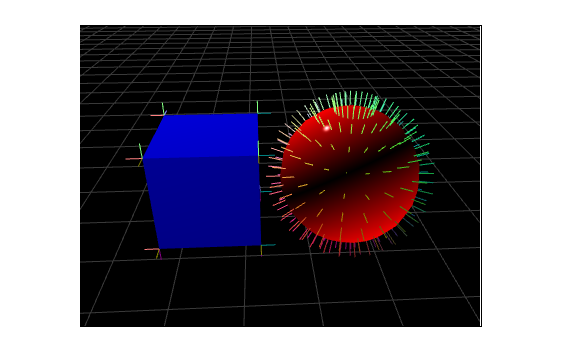
\includegraphics[width=6cm]{NORMALS.PNG}
	\caption{Image showing the normals of a sphere and square.}
\end{figure}

Clearly we can see in the figure above that the cuboid and sphere have different normals to their surfaces and it goes without saying that this difference in normals will affect how the light on the different points of the surface (with different normals) will interact, we can see this in the diagram from the fact the lighting on the cuboid is far more consistent than the lighting on the sphere (it is not coincidental that the cuboids normals are also more consistent).\\

Specifically this type of lighting is called directional lighting, roughly summarised directional lighting means that whichever part of the surface is closest to a light source is the brightest and without normals we would be unable to determine the direction of the surfaces normals and thus we would be unable to determine which part of the surface is receiving the most light.\\
\item Suppose $\text{drawBox(m)}$ is a function to draw a transformed box according to the transformation matrix $m$. That is, if $M$ is a rotation matrix, the function will draw a rotated box. 
\subitem a. Explain the meaning of the following code segment and state the result obtained:
\subitem $\text{				m.setTranslate(20.0, 0.0, -30.0);}$
\subitem $\text{				m.rotate(angle, 2.0, 0.0, 0.0);}$
\subitem $\text{				drawBox(m);}$\\
\subitem This function draws a box which has been roated angle degrees in the x-axis, then translated 20 units in the positive x-direction and 30 units in the negative z-direction. Below I will explain why this occurs, and why it occurs in that order.
\subitem m.setTranslate essentially creates a new transformation matrix using the parameters \subitem provided and stores the value in m, so our new transformation matrix after the line $\text{m.setTranslate(20.0, 0.0, -30.0);}$ is carried out will be:\\
\subitem $\begin{bmatrix}
    1   & 0 &0  & 20 \\
    0   & 1 & 0 & 0 \\
    0  & 0 & 1 & -30 \\
    0  & 0 & 0 & 1
\end{bmatrix}$.\\
\subitem Thus at this point $m$ represents the above translation matrix which translates 20 units in the direction of the x-axis and -30 units in the direction of the z-axis.\\ Then when we perform m.rotate(angle, 2.0, 0.0, 0.0); we are multiplying (multiplying from the left) our transformation matrix by  a rotation matrix. Specifically, this is the rotation matrix which performs a rotation of 'angle' degrees around the rotation axis (2.0, 0.0, 0.0). The rotation matrix will appear as \subitem follows (where $\theta$ is the angle specified): 
\subitem $\begin{bmatrix}
    1  & 0 &0  & 0 \\
    0   & \cos (\theta) & -\sin (\theta) & 0 \\
    0  & \sin (\theta) & \cos (\theta) & 0 \\
    0  & 0 & 0 & 1
\end{bmatrix}$.\\
\subitem However, what I have perhaps not made clear is that we are performing the rotation \subitem first folowed by the translation (the translation is set first due to the way that matrix \subitem multiplication works) So our transformation matrix will appear as follows:
\subitem $\begin{bmatrix}
    1   & 0 &0  & 20 \\
    0   & 1 & 0 & 0 \\
    0  & 0 & 1 & -30 \\
    0  & 0 & 0 & 1
\end{bmatrix} \cdot \begin{bmatrix}
    1  & 0 &0  & 0 \\
    0   & \cos (\theta) & -\sin (\theta) & 0 \\
    0  & \sin (\theta) & \cos (\theta) & 0 \\
    0  & 0 & 0 & 1
\end{bmatrix} = \begin{bmatrix}
    1  & 0 &0  & 20 \\
    0   & \cos (\theta) & -\sin (\theta) & 0 \\
    0  & \sin (\theta) & \cos (\theta) & -30 \\
    0  & 0 & 0 & 1
\end{bmatrix} $
\\
\subitem Thus if we were to perform the transformation on a set of co-ordinates it would appear \subitem as follows:
\subitem $ \begin{bmatrix}
    1  & 0 &0  & 20 \\
    0   & \cos (\theta) & -\sin (\theta) & 0 \\
    0  & \sin (\theta) & \cos (\theta) & -30 \\
    0  & 0 & 0 & 1
\end{bmatrix}  \cdot \begin{bmatrix}
    x \\
    y \\
    x \\
     1
\end{bmatrix} = \begin{bmatrix}
    x + 20 \\
    \cos(\theta)y - \sin(\theta)z \\
    \sin(\theta)y + \cos(\theta)z - 30 \\
     1
\end{bmatrix}$
\subitem Clearly we can see that the code segment has produced a transformation matrix which \subitem will rotate the co-ordinates about the x-axis followed by translating it 20 units in the  \subitem positive  x-direction and 30 units in the negative z-direction.
\subitem Finally the drawBox function is called with the transformation matrix passed as a \subitem parameter, the transformation is then performed on the box .
\\
\\
\\
\subitem b. Explain whether you will get the same result if m.rotate() has been replaced by \subitem m.setRotate().
\subitem You will not get the same result, when using the setRotate function the transformation matrix is set to the matrix associated with the parameters. Specifically this matrix will be (where) $theta$ is the angle we're rotating by):
\subitem  $m  \cdot \begin{bmatrix}
    1  & 0 &0  & 0 \\
    0   & \cos (\theta) & -\sin (\theta) & 0 \\
    0  & \sin (\theta) & \cos (\theta) & 0 \\
    0  & 0 & 0 & 1
\end{bmatrix} = \text{ new transformation matrix } m$
\subitem This differs for the m.rotate(angle, 2.0, 0.0, 0.0) function as m.rotate multiplies the existing transformation matrix ($m$) by the rotation matrix, compared with m.setRotate(angle, 2.0, 0.0, 0.0) effectively overriding the existing transformation matrix to create an entirely matrix based upon the parameters provided.

\subitem Clearly if we to use the setRotate method we would no longer be adapting the current state of $m$ and we are instead setting a new matrix entirely based upon the parameter values provided and setting it to $m$.
\subitem  $m  = \begin{bmatrix}
    1  & 0 &0  & 0 \\
    0   & \cos (\theta) & -\sin (\theta) & 0 \\
    0  & \sin (\theta) & \cos (\theta) & 0 \\
    0  & 0 & 0 & 1
\end{bmatrix}$
\subitem As such if we use the .setRotate() method any value of $m$ prior to using the method will be ignored, and the drawBox function would simply draw a rotated box rather than rotated box that has then been translated.
\end{enumerate}
\end{document}